\documentclass[a4paper]{article} 
\usepackage[14pt]{extsizes} % для того чтобы задать нестандартный 14-ый размер шрифта 
\usepackage[utf8]{inputenc} 
\usepackage[russian]{babel} 
\usepackage{amsmath,amsfonts,amssymb,amsthm,mathtools} 
\usepackage[left=20mm, top=15mm, right=15mm, bottom=15mm, nohead, footskip=10mm]{geometry} % настройки полей документа 

\begin{document} % начало документа 
% НАЧАЛО ТИТУЛЬНОГО ЛИСТА 
\begin{center} 
\hfill \break 
\large{Санкт-Петербургский Политехнический университет имени Петра Великого}\\ 
 
 \hfill \break 
\hfill\break 
\hfill \break 
\hfill \break 
\hfill \break 
\large{Отчёт по лабораторной работе №1}\\ 
\hfill \break 
\large{Тема: Интерполяционные  полиномы    приближения  табличных  функций. } 
\hfill \break 
\hfill \break 
 
\hfill \break 
\hfill \break 
\\ 
\hfill \break 
\hfill \break 
\end{center} 


\normalsize{ 
\begin{tabular}{cccc} 
Студент & : & Алексеева Мария Сергеевна\\\\ 
Группа & : & 5030103/00003 \\\\ 
Преподаватель & : & Козлов Константин Николаевич \\\\ 
\end{tabular} 
}\\ 
\hfill \break 
\hfill \break 
\hfill \break 
\begin{center} Санкт-Петербург 2022 \end{center} 
\thispagestyle{empty} % выключаем отображение номера для этой страницы 
 
% КОНЕЦ ТИТУЛЬНОГО ЛИСТА 
\newpage 
	
\section{Формулировка задачи и её формализация} 
Задача: Построить полином в форме Лагранжа на Чебышевской и произвольной со сгущением на выбранном интервале сетке для двух функций: $ y(x) = x - sin(x)$ и $ y(x) = 3sign(x)x^{4}-8x^{3}-18x^{2}+6$ на интервале $[-1.3;-0.9;0.14;0.53;0.8;1.05]$. Исследовать влияение количества узлов сетки и гладкости функции на интерполяционную ошибку.
\section{Алгоритм метода и условия его применимости} 
\subsection{Интерполяционный полином Лагранжа} 
Зададим некоторую функцию и, выбрав некоторый интервал, вычисляем значения функций для уже заданного массива х. 
Интерполяционный полином в форме Лагранжа имеет общий вид:\\

\begin{center}
$L_n (x) =\sum_{i=0}^n y_i \Phi_i(x)\sum$, где $ \Phi_i = \delta_i(x){}_j$ 
\end{center}

\begin{flushleft}
С помощью некоторых преобразований мы приходим к виду:\\
\end{flushleft}
\begin{center}
$L_n (x) =\sum_{i=0}^n y_i \prod\limits_{ {k = 0}, {k \neq i} }^n \frac{x-x_k}{x_i-x_k}$
\end{center}
\subsection{Условия применимости}
Функция, которую мы будем интерполировать должна быть непрерывна. Поэтому для того, чтобы реализовать интерполяцию полиномом Лагранжа возьмем подходящие функции. Интерполирование полинома может происходить лишь на упорядоченной сетке. Узлы должны быть попарно различными.
\subsection{Виды сеток для массива х} 
\textbf{Неравномерная:} 
Такая сетка имеет лишь упорядоченность, то есть $ x_0 = a < x_1<x_2<...<x_n = b$, в частном случае решения моей задачи была выбрана неравномерня сетка со сгущение в районе середины интервала.
Сгущение получено путем добавления в середину равномерной сетки дополнительного разбиения. Т.е. создается массив из n равноотстающих узлов, в нем выбирается два элемента с номерами $round(n/2)$ и $round(n/2)-1$. Эти элементы объявляются границами нового массива, в котором также будет n элементов. В конечном итоге, сетка со сгущением будет получена путем "склеивания", упорядочивания и удаления повторяющихся элементов из двух этих массивов.  \\ 
\textbf{Чебышевская сетка:} Сетка строится по принципу того, что ее узлами являются корни полинома Чебышева\\

 
\section{Предварительный анализ задачи} 
Интерполяционный полином Лагранжа имеет степень на 1 меньше, чем размер рассматриваемого нами массива х и у. И требуется выполнение условий интерполяции: 
\begin{center}
$ \phi(x_i) = y_i$ 
\end{center}
\section{Тестовый пример с расчётами} 
В качестве примера  можем рассмотреть некоторый массив с равномерной сеткой  $ x_0=1 $ на отрезке [1, 3].\\
Тогда зададим шаг $ h = 1$. Таким образом массив х:\\
 $x_i = [1, 2, 3, 4]$\\
Пусть функция будет задаваться формулой:  $y = x+ln(x)+0.5$. Таким образом массив для у:\\
$ y_i = [1.5, 3.2, 4.6, 5.9]$\\
А теперь найдем полином Лагранжа для заданной функции. \\
\begin{flushright}
$ L_3(x) = 1.5 \frac{(x-2)(x-3)(x-4)}{(1-2)(1-3)(1-4)}+3.2\frac{(x-1)(x-3)(x-4)}{(2-1)(2-3)(2-4)}+4.6\frac{(x-1)(x-2)(x-4)}{(3-1)(3-2)(3-4)}+5.9\frac{(x-1)(x-2)(x-3)}{(4-1)(4-2)(4-3)}$\\ 
\begin{center}
$L_3(x)= \dfrac{1}{30}x^3-\dfrac{7}{20}x^2+\dfrac{151}{60}x-\dfrac{7}{10}$\\
Рассмотрим значение функции и значение полинома в выбранной точке $x = 1.5$\\
$y(x)= 2,40547$ - для функции, $L_3(x) =2.4$ - для полинома. Погрешность равна 0,00547, т.о. видим, что полином построен корректно.
\end{center}
\end{flushright}


 
\section{Подготовка контрольных тестов для иллюстрации метода} 
Для примера будут реализованы графики одной функции с разными сетками: произвольной со сгущением на интервале в середине отрезка и Чебышевской.
Гладкая функция $ y(x) = x - sin(x)$ и функция с разрывом  $ y(x) = 3sign(x)x^{4}-8x^{3}-18x^{2}+6$ будут построены на интервале $[-1.3;-0.9;0.14;0.53;0.8;1.05]$, также будут построены полиномы Лагранжа для этих функций в заданных из отрезка узлах. 
Далее будут проведены исследования, чтобы проверить зависимость ошибки интерполяции в узлах Чебышевской и произвольной сетки со сгущением. Сетки будут построены с концами отрезков $[-1.3; 1.05]$.
  
\newpage
\section{Модульная структура программы} 
 
\begin{figure}[h!]
\begin{center}
 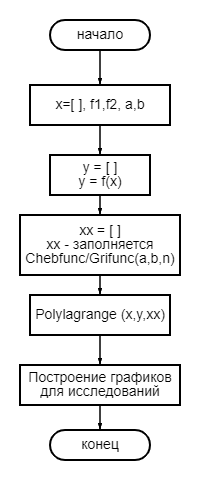
\includegraphics[scale=0.7]{diagram (5).png} 
 \end{center}
\caption{Блок-схема кода программы} \label{Рис1}
\end{figure}

\begin{figure}[h!]
\begin{center}
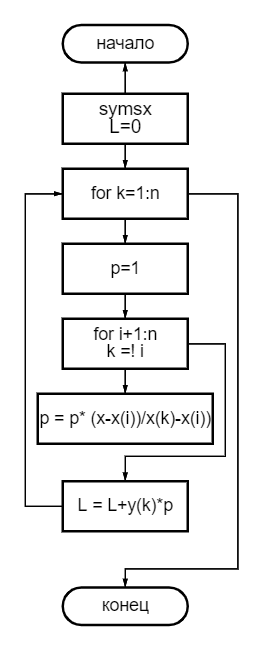
\includegraphics[scale=0.7]{diagram (6).png} 
\end{center}
\caption{Блок-схема кода полинома Лагранжа } \label{Рис2}
\end{figure}

\newpage
\section{Численный анализ решения задачи}
\subsection{Задание функции и массивов} 
По условию заданы функции $ y = x+sin(x)$ и $ y(x) = 3sign(x)x^{4}-8x^{3}-18x^{2}+6$, рассмотрим их на отрезке $[-1.3;-0.9;0.14;0.53;0.8;1.05]$. Тогда для заданной функции строим полином Лагранжа с неравномерной сеткой, таким образом, получаем график на рисунке \ref{Рис3}.
\begin{figure}[h!]
\begin{center}
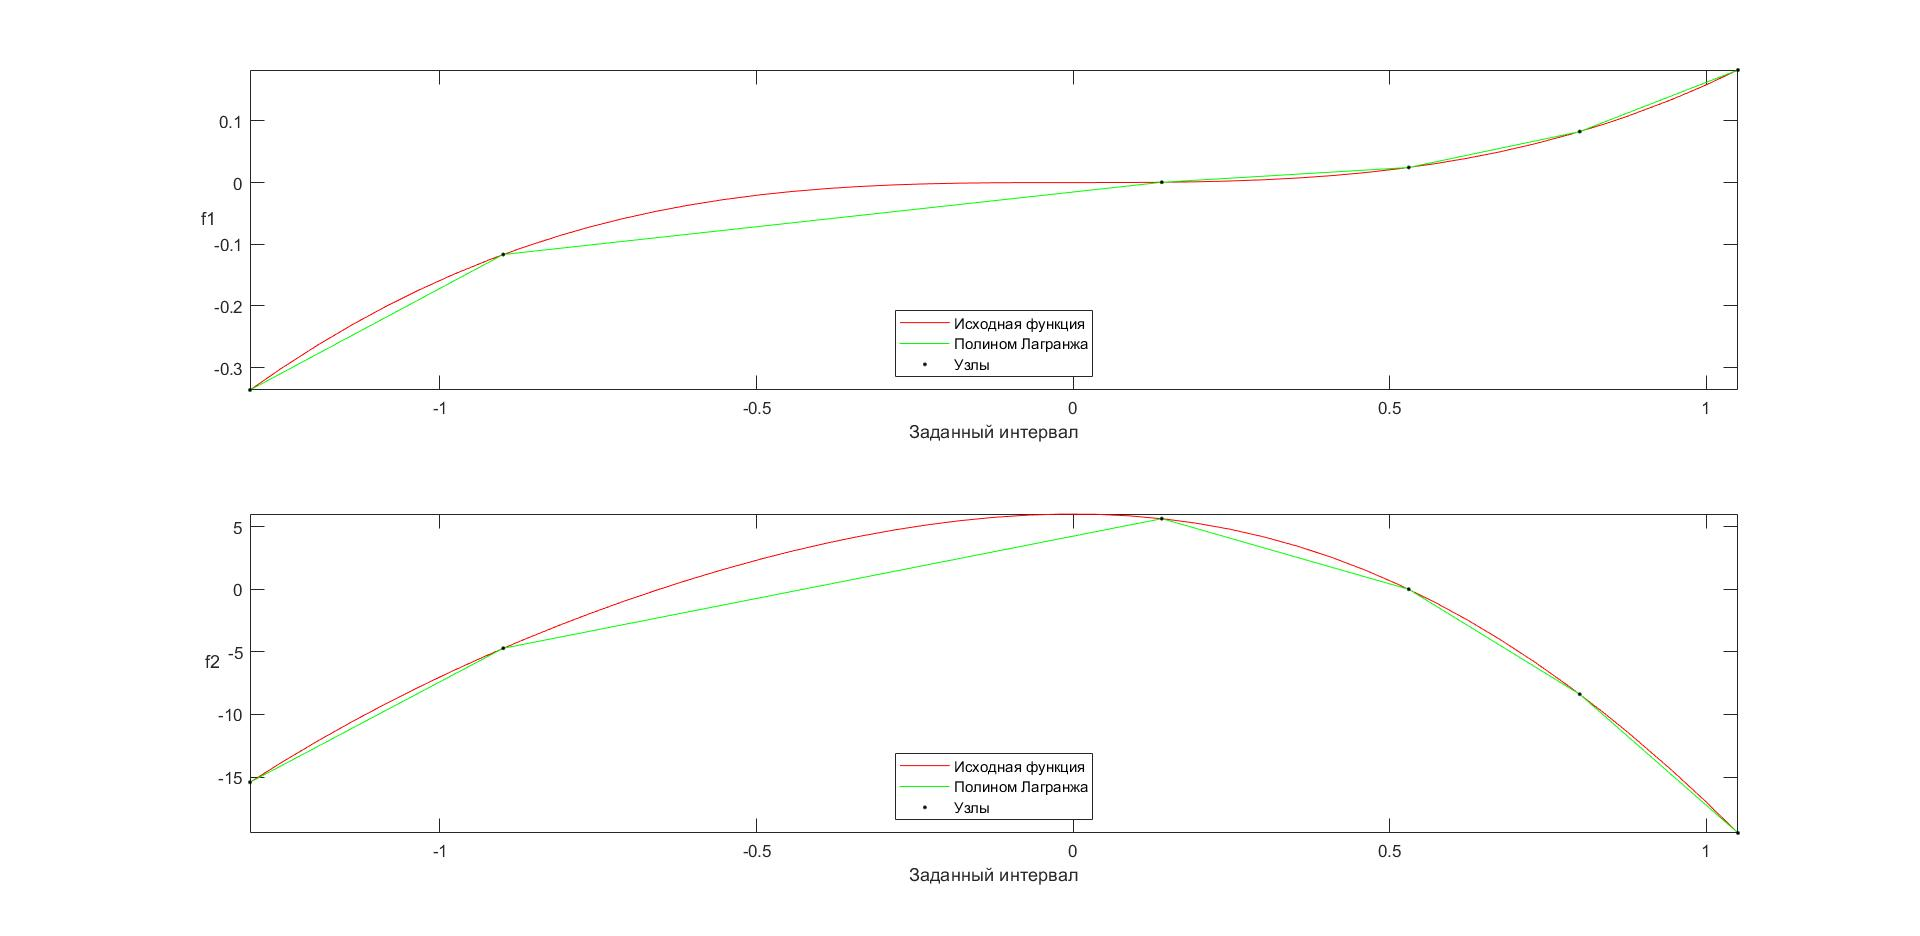
\includegraphics[scale=0.3]{функции.jpg} 
\end{center}
\caption{график полинома Лагранжа и исходной функции на заданном интервале} \label{Рис3}
\end{figure}\\

\newpage

\section{Исследование влияния количества узлов на интерполяционную сходимость} 
На рисунке \ref{Рис4} мы видим, что максимальная погрешность при увеличении узлов сетки возрастает, причем монотонно, как для гладкой, так и не для гладкой функций. На графике отображается максимальная ошибка интерполяции для заданного количества узлов. Можно заметить, что погрешность принимает достаточно большое значение даже при маленьком количестве узлов. Это происходит потому что интерполяция ведется на равномерной сетке со сгущением(сгущение также равномерно), а как мы знаем, на концах отрезков проявляется недостаток интерполяции на равномерной сетке - большое значение ошибки интерполяции. Так как мы делаем сгущение в равномерной сетке по центру, то нехватка узлов по краям никак не компенсируется и ошибка на концах все равно является большой.  Можно сделать вывод, что для равномерной сетки неэффективно использовать сгущение в центре.\\
Исходя из теоретической части,чтобы получить меньшую ошибку, следует использовать другую сетку, а именно Чебышевскую.
\begin{figure}[h!]
\begin{center}
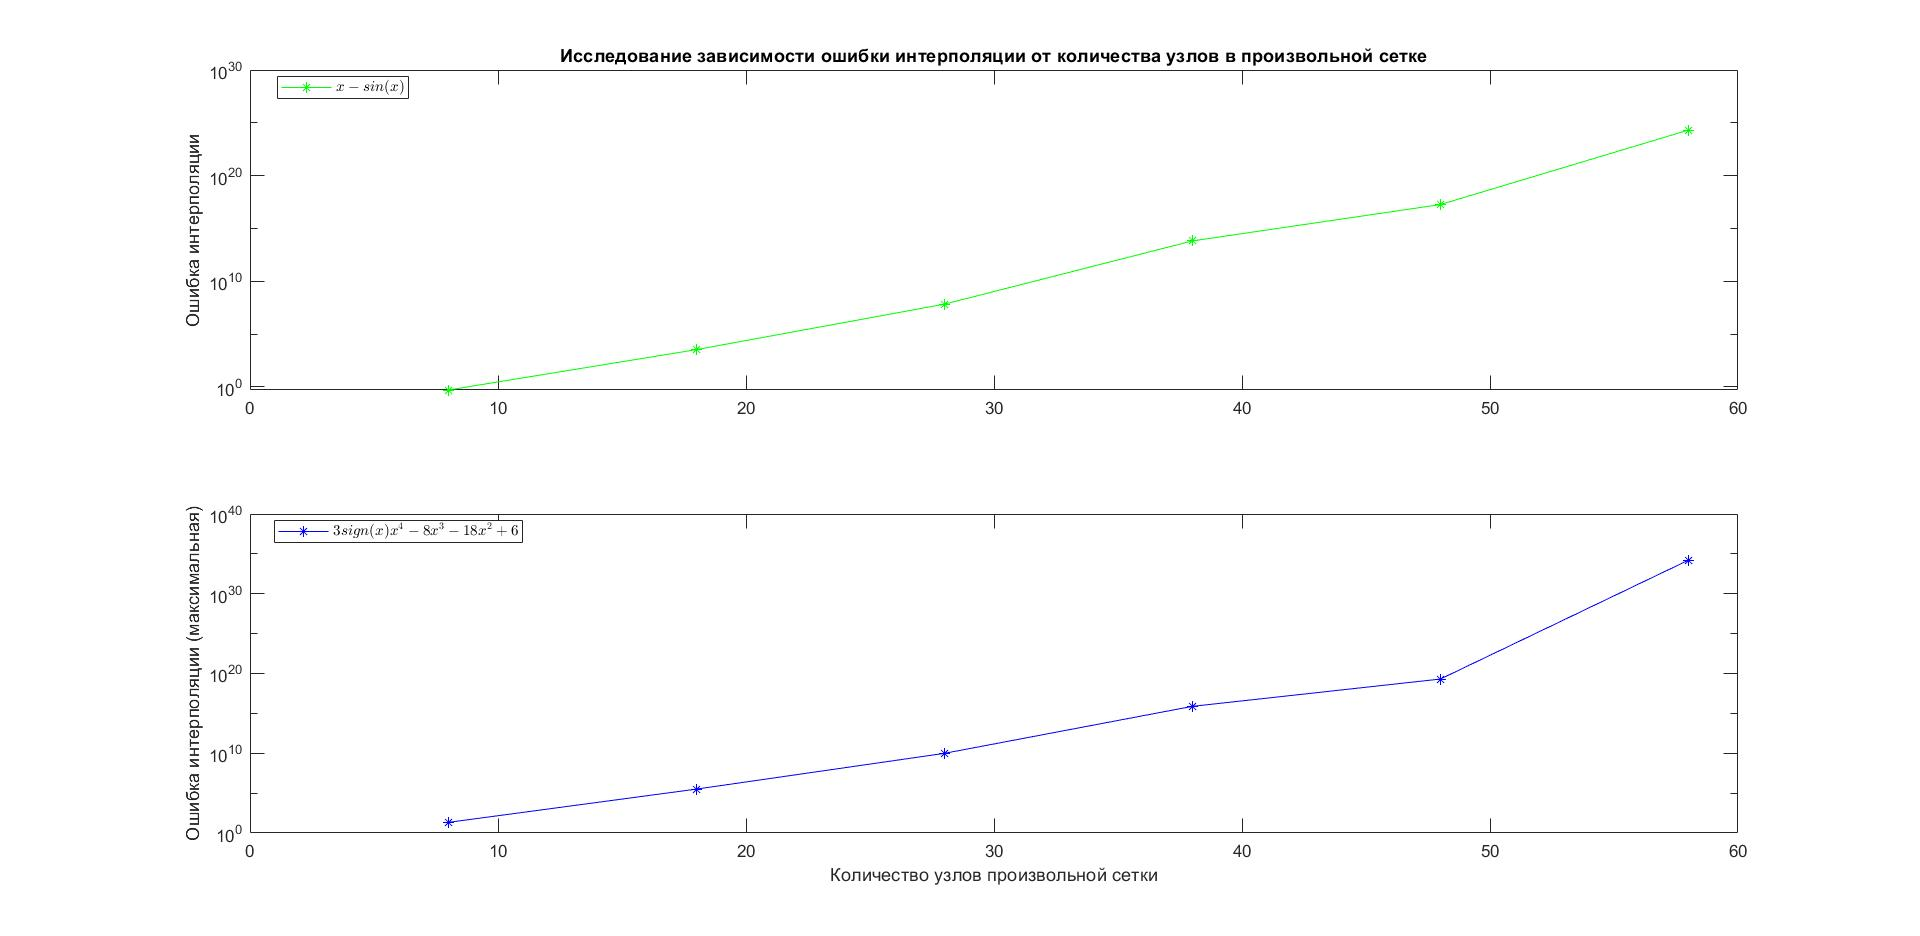
\includegraphics[scale=0.3]{кол-во узлов Произвольная.jpg} 
\end{center}
\caption{Кол-во узлов, произвольная сетка} \label{Рис4}
\end{figure}\\

На рисунке 5 мы видим, что при увеличении узлов Чебышевской сетки погрешность уменьшается, однако в определенном значении количества узлов наблюдается ее резкое возрастание. Видно, что погрешность действительно меньше, чем при построении полинома на  сетке со сгущением. 
\begin{figure}[h!]
\begin{center}
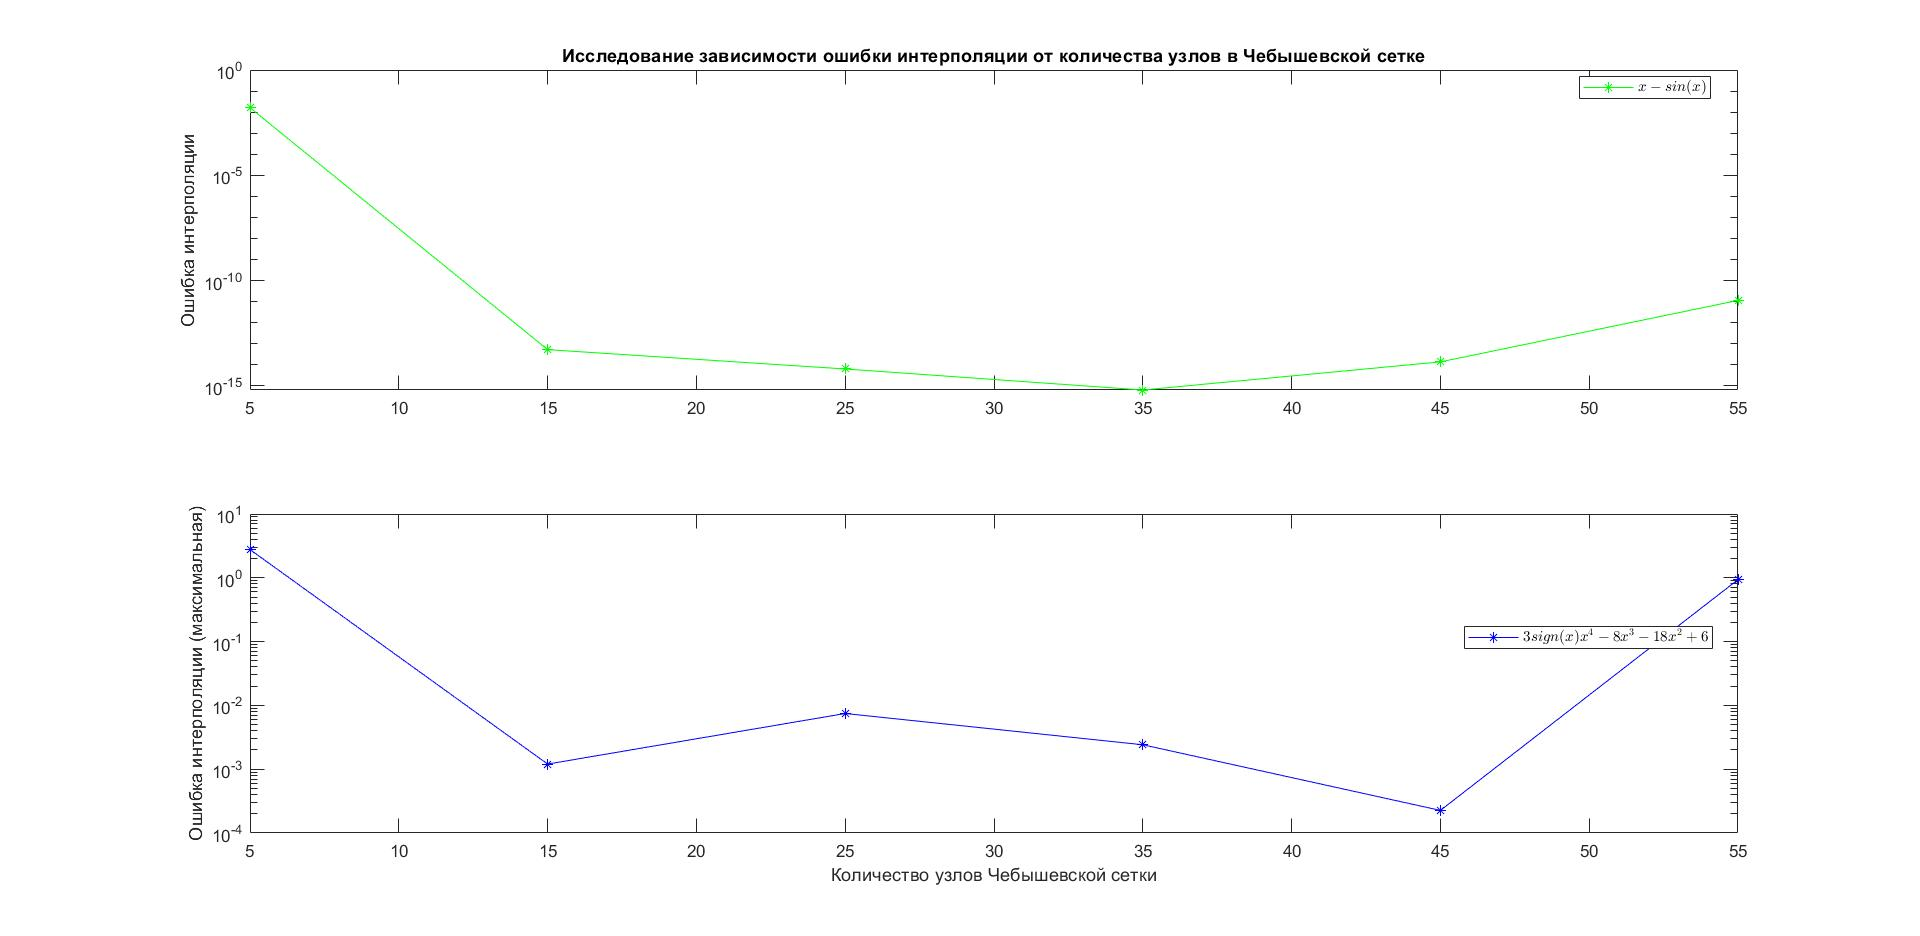
\includegraphics[scale=0.3]{кол-во узлов Чебышев.jpg} 
\end{center}
\caption{Кол-во узлов, Чебышевская сетка} \label{Рис5}
\end{figure}\\

\newpage
\section{Исследование влияния гладкости на интерполяционную сходимость} 
Возьмем гладкую функцию и функцию, которая имеет разрыв производной.
 \begin{center}
$ y = x+sin(x)$  - гладкая функция\\
$ y(x) = 3sign(x)x^{4}-8x^{3}-18x^{2}+6$ - негладкая функция
\end{center}


 

\textbf{Чебышевская сетка}
\begin{figure}[h!]
\begin{center}
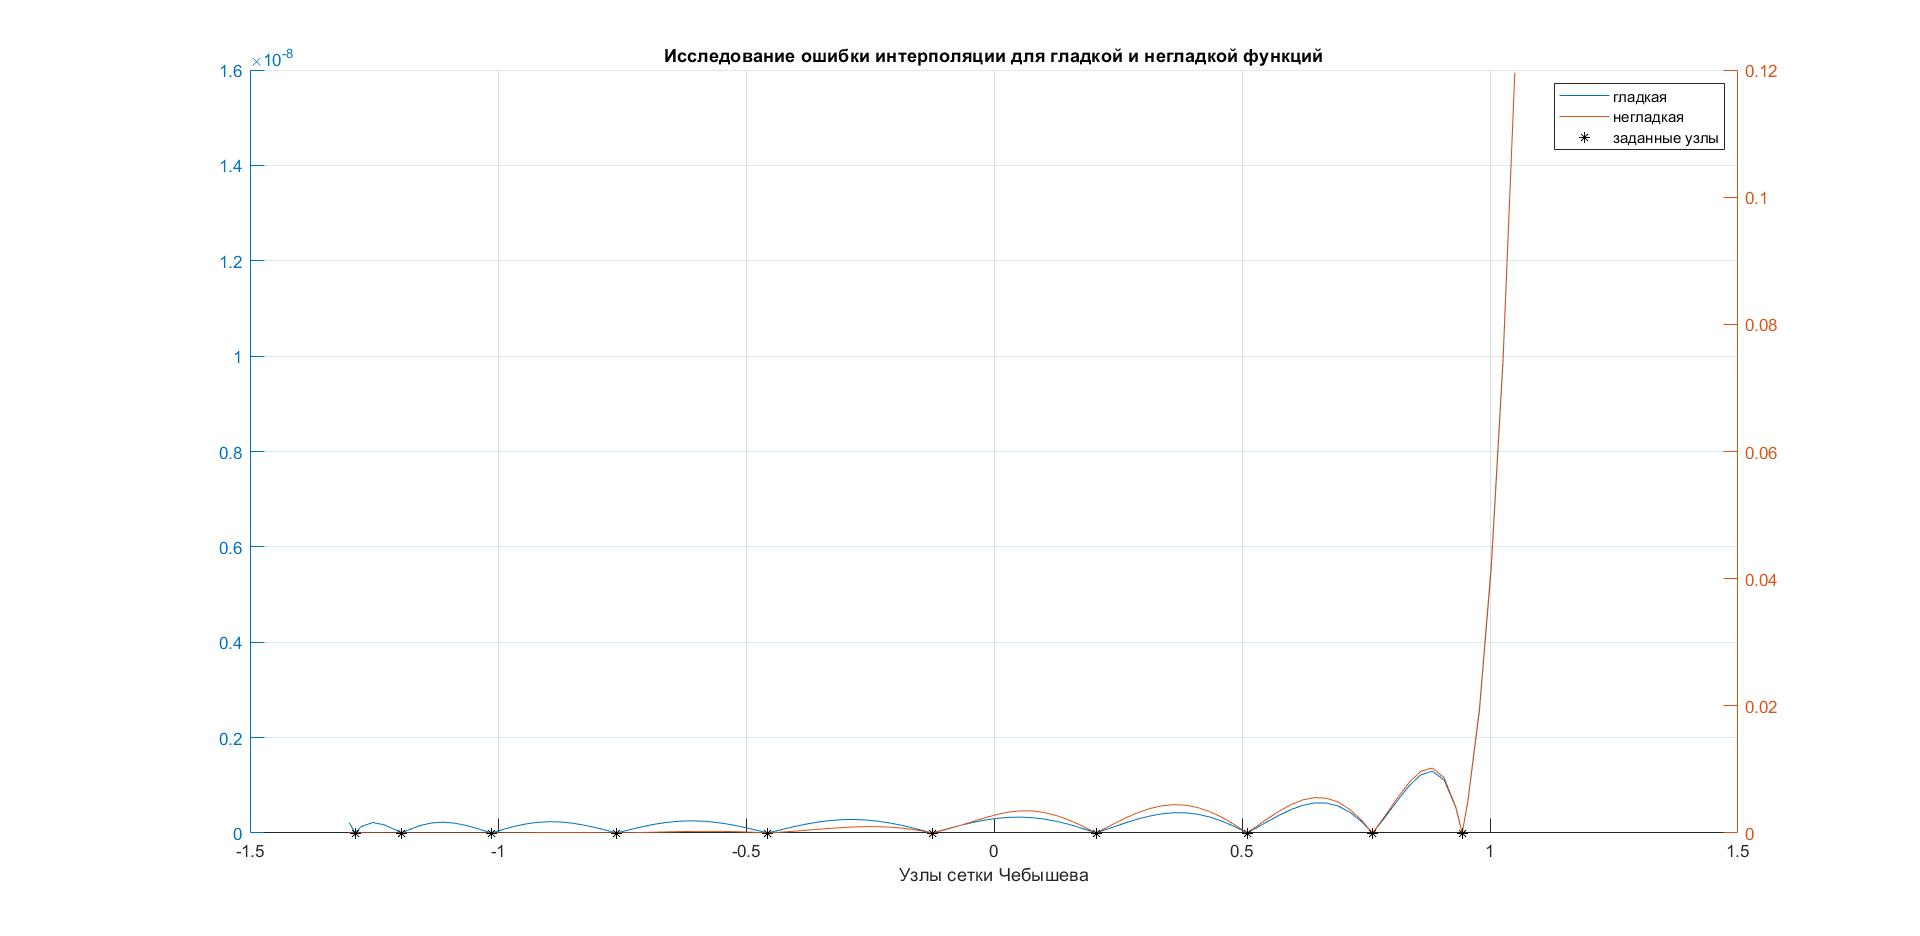
\includegraphics[scale=0.3] {гладкая и негладкая чебышев.jpg} 
\end{center}
\caption{Гладкая и негладкая на Чебышевской сетке} \label{Рис5}
\end{figure}\\

\textbf{Произвольная сетка}
\begin{figure}[h!]
\begin{center}
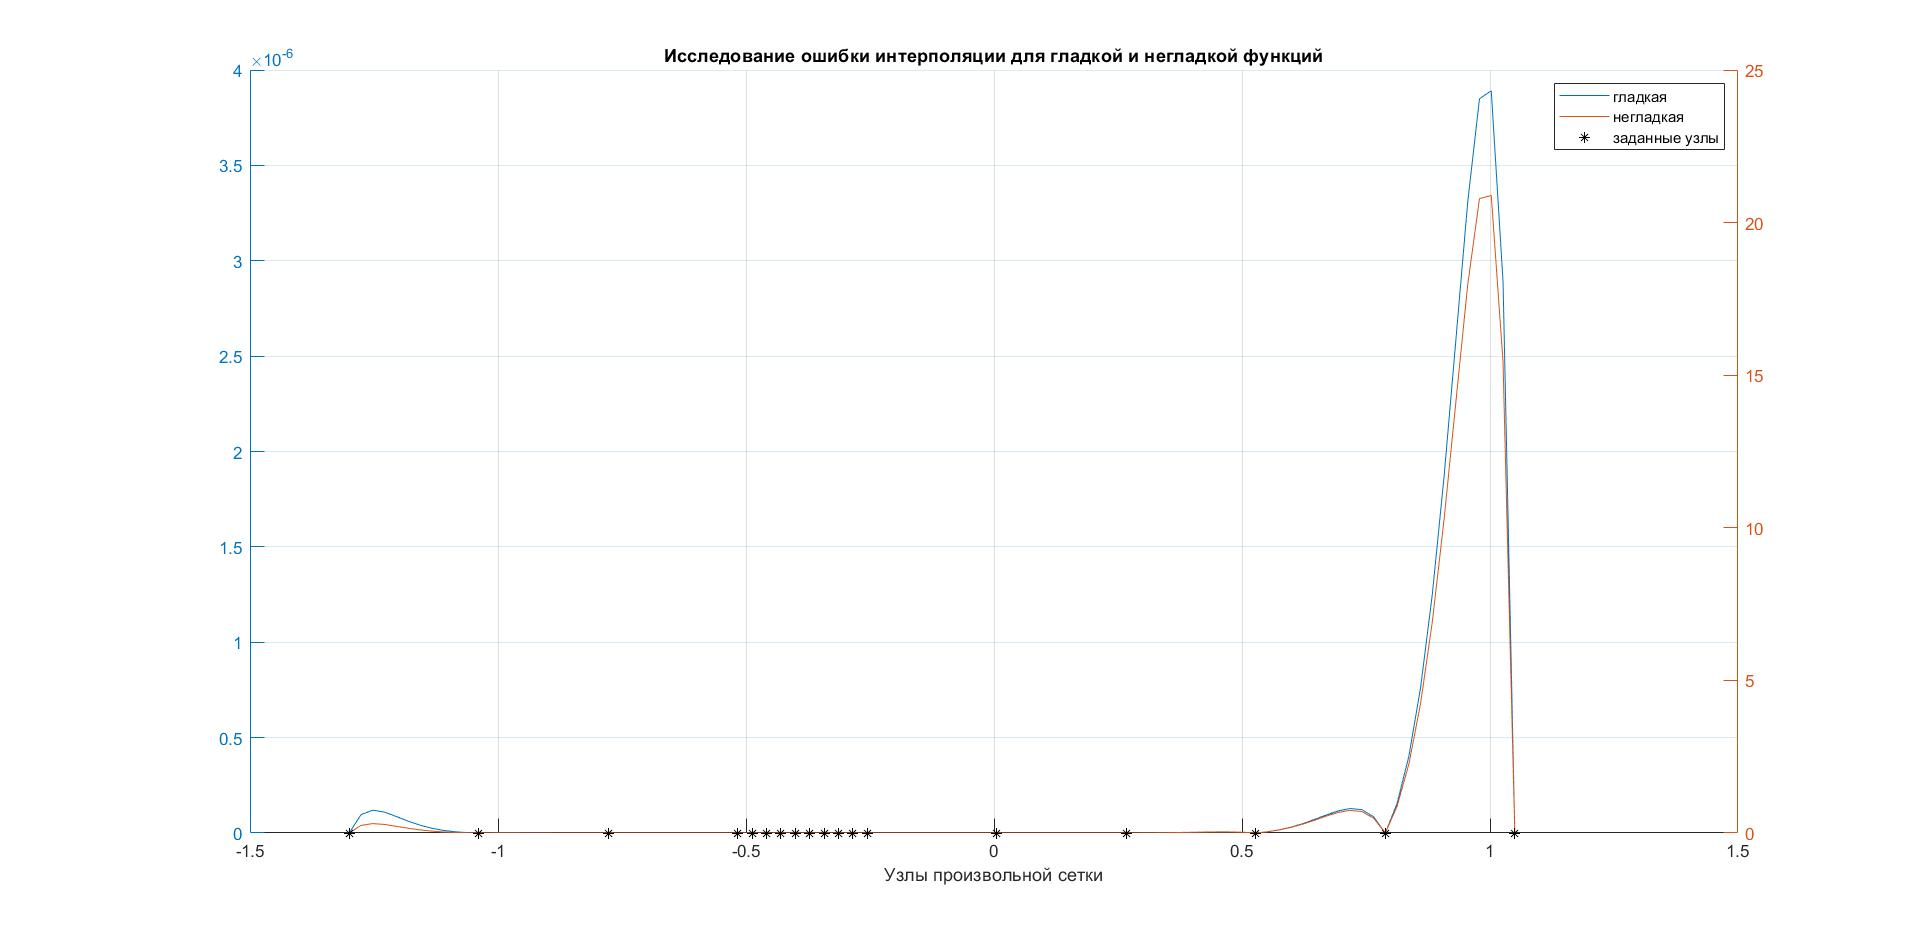
\includegraphics[scale=0.3]{гладкая и негладкая произвольная.jpg} 
\end{center}
\caption{Гладкая и негладкая на произвольной сетке} \label{Рис6}
\end{figure}\\
Как видно из графиков рисунки \ref{Рис5}  и \ref{Рис6} ошибка интерполяции на гладкой функции меньше, чем на функции с разрывом. На произвольной сетке на концах видно возрастание ошибки, что было освещено в предыдущих пунктах.

\newpage
\section{Краткие выводы} 

\begin{itemize}
  \item Интерполяционный полином Лагранжа дает хорошее приближение к исходному графику, если подобрать верную сетку 
  \item На равномерной сетке можно заметить большое отклонение от заданной функции на концах отрезка, но во-первых это можно исправить, построив полином на более "хорошей" сетке, во-вторых максимальная ошибка далека от остальных значений ошибки(которые являются достаточно малыми) $=>$ построение можно считать достаточно корректным. Однако построение на сетке со сгущением в середине отрезка все же не является достаточно эффективным.
  \item При сравнении гладкой функции и функции с разрывом в производной было понято, что интерполяцию лучше проводить для гладкой функции, т.к. она даст лучший результат с меньшим значением ошибки.
  \item Также мною было замечено то, что при построении достаточного большого количества узлов программа выполняется медленно, что обусловлено тем, что полином Лагранжа каждый раз считается "с нуля" и все предыдущие вычисления с меньшим количеством узлов не запоминаются.
   
\end{itemize}


\end{document} % КОНЕЦ ДОКУМЕНТА !

